
%(BEGIN_QUESTION)
% Copyright 2014, Tony R. Kuphaldt, released under the Creative Commons Attribution License (v 1.0)
% This means you may do almost anything with this work of mine, so long as you give me proper credit

Beregn alle spenninger og alle strømmer i denne kretsen, gitt komponentverdiene og viklingstallene i transformatoren:

$$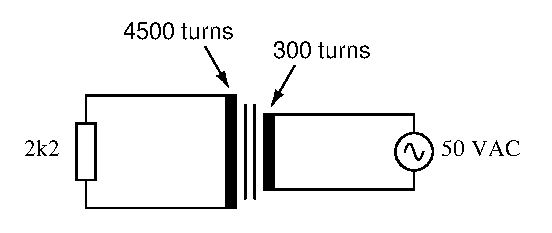
\includegraphics[width=15.5cm]{i01239x01.eps}$$

\underbar{file i01239}
%(END_QUESTION)





%(BEGIN_ANSWER)

$V_R =$ 750 V

$I_R =$ 340.9 mA

\vskip 5pt

$V_{source} =$ 50 V

$I_{source} =$ 5.114 A

%(END_ANSWER)





%(BEGIN_NOTES)

Denne oppgaven tester elevenes evne til å relatere viklingsforhold til spennings- og strømforhold i en transformator. Symbolbruken her er vanlig i Europa, men mindre vanlig i USA.

%INDEX% Elektronikkrepetisjon: transformatorforhold

%(END_NOTES)

